%!TEX root = ../thesis.tex
%*******************************************************************************
%*********************************** Research Timelines *****************************
%*******************************************************************************



\chapter{Research Timeline}  %Title of the Research Timeline

\ifpdf
    \graphicspath{{ResearchTimeline/Figs/Raster/}{ResearchTimeline/Figs/PDF/}{ResearchTimeline/Figs/}}
\else
    \graphicspath{{ResearchTimeline/Figs/}{ResearchTimeline/Figs/}}
\fi

The following chapter talks about the research activity timeline conducted for a duration of 2 and half years. 
The plan is subject to change based on any deviation which will be attempted to be covered in the risk analysis 
section. The recent tasks are provided in depth in contrast to later tasks which will be more open ended 
as it reliant to the results from preceding tasks. 

\begin{figure}[htbp!] 
  \centering    
  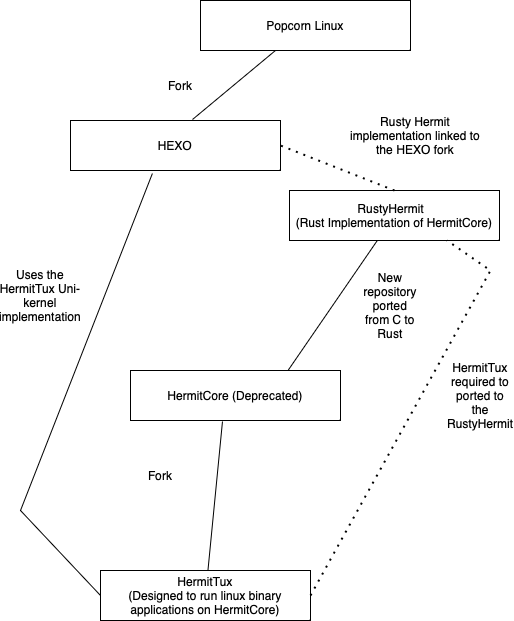
\includegraphics[width=0.6\textwidth]{PlannerActivity}
  \caption[Planner]{High-level overview of the porting efforts}
  \label{fig:PlannerPorting}
  \end{figure}

Before starting a heavy discussion of the plan and experiment a few things that should cleared out before starting would be 
the higher overview of the experiment and why certain porting efforts are required. The Segments would be classified into: 
\begin{enumerate}
  \item Porting Unikernel implementation 
  \item Porting CheriOS to a Uni-kernel
\end{enumerate}

\subsubsection{Porting Unikernel implementation}
The Uni-kernel implementation used for the following PhD would be RustyHermit 
which is Rust implementation of the Uni-kernel project Hermit-core. The reason 
RustyHermit was selected is because the Hermit-core project is deprecated and 
the recent version of the project in the RustyHermit repo. To give a better 
background the HEXO paper \cite{HEXO} which uses Popcorn Linux to offload 
tasks to a potato machine (i.e raspberry pi) which uses the HermitTux Uni-kernel (This 
is a fork for the Hermit-core Uni-kernel). The HermitTux fork of HermitCore is used to 
run Linux ABI binary files on a Uni-kernel. To ensure we can continue working with the
planned experiments. It would recommended to port HermitTux to RustyHermit to ensure we 
can sync the new version of HermitTux with the latest changes from RustyHermit. Fig ~\ref{fig:PlannerPorting}
 provides the visual description of the following paragraph. 

\subsubsection{Porting CheriOS to a Uni-kernel}
The selected TAG based architecture would be CHERI due to ease to acquiring of hardware 
for performance (i.e the ARM based CHERI morello). The official supported OS for 
the CHERI hardware is the CheriBSD \cite{CHERIBSD}. While doing experiments it 
would save a lot of time initially just porting the required kernel modules to 
RustyHermit.

\subsubsection{Hardware requirements}
Initially from the month of January 2023 they would tested locally on 
my personal of machine, but over the semester 
\begin{enumerate}
  \item 1 Cheri Morello machine 
  \item 2 Bare-metal x86 machines
  \item 2 FPGAs (For testing new architectures)
  \item 2 ARM based machines
  \item Rack space for setting up the machines 
\end{enumerate}

\subsubsection{The tasks are split into the following tags:}
\begin{enumerate}
  \item Porting 
  \item Setup
  \item Development
  \item Exploration 
  \item Technical discussion 
  \item Writing
  \item Testing
  \item Publishing
  \item Thesis
  \item Break
  \item Other
\end{enumerate}

% \subsection{More context}
% This section is split by a month by month planner to help keep tracks of tasks. 

\subsection{Year 2}
This section is split by a month by month planner to help keep tracks of tasks. 
\begin{landscape}
\begin{figure}[htbp!] 
  \centering    
  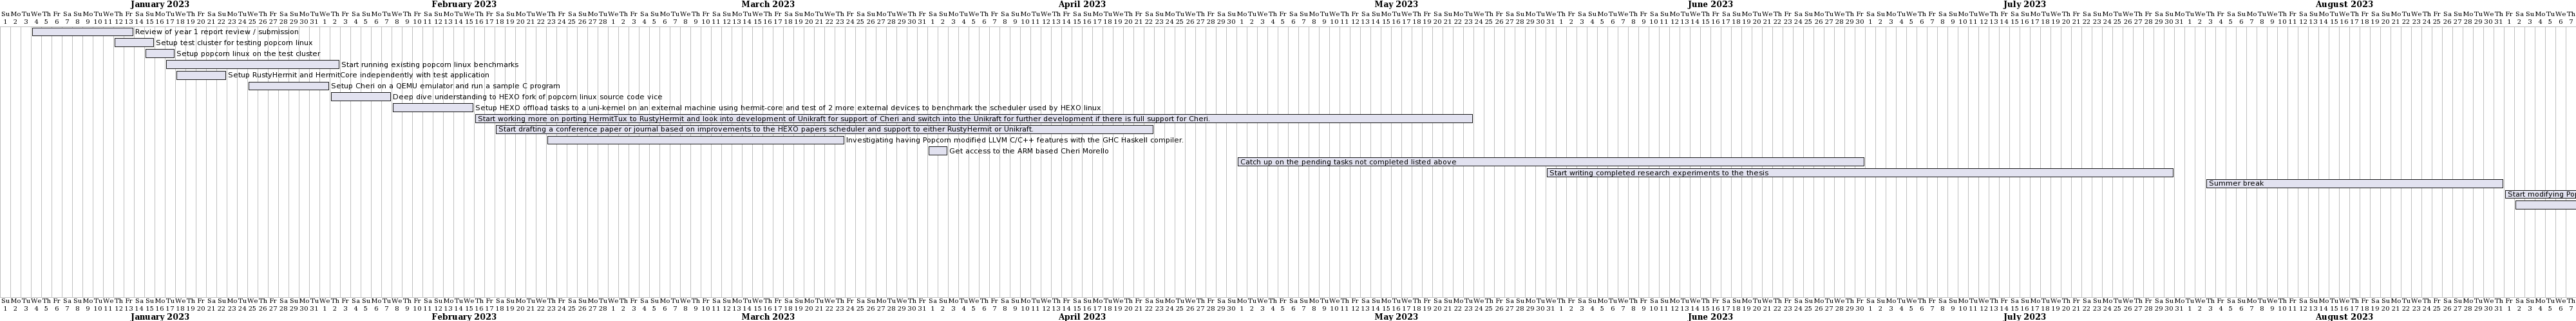
\includegraphics[width=6\textwidth]{gnatt}
  \caption[Planner]{Gantt Chart till summer 2023}
  \label{fig:Gantt Chart}
  \end{figure}
\end{landscape}

\subsubsection{January 2023}
The high level overview being that most of the setups for the upcoming experiments
are complete. 
\begin{enumerate}
    \item (\(Review\)) Review of year 1 report submitted 
    \item (\(Setup\)) Setup test cluster for testing popcorn linux 
    \item (\(Setup\)) Setup popcorn linux on the test cluster
    \item (\(Testing\)) Start running existing popcorn linux benchmarks 
    \item (\(Setup\)) Setup RustyHermit and HermitCore independently with test application 
    \item (\(Setup\)) Setup Cheri on a QEMU emulator and run a sample C program 
  \end{enumerate} 


  \subsubsection{February 2023}
  \begin{enumerate}
    \item (\(Exploration\)) Deep dive understanding to HEXO fork of popcorn linux source code vice.
    \item (\(Setup\)) Setup HEXO offload tasks to a uni-kernel on an external machine using hermit-core 
    and test of 2 more external devices to benchmark the scheduler used by HEXO linux. 
    \item (\(Porting\)) Start working more on porting HermitTux to RustyHermit and look into 
    development of Unikraft for support of Cheri and switch into the Unikraft for further 
    development if there is full support for Cheri. 
    \item (\(Writing, Publishing\)) Start drafting a conference paper or journal based on improvements to the HEXO papers 
    scheduler and support to either RustyHermit or Unikraft. 
  \end{enumerate}

  \subsubsection{March 2023}
  \begin{enumerate}
    \item (\(Porting\)) Start porting either RustyHermit or Unikraft to support the Cheri Architecture. (The following sub-section is assuming 
          RustyHermit is selected).
          \begin{enumerate}
            \item Making a rust based clone of Hermitux on the rust based rusty-hermit. 
            \item Merging certain C libraries from CheriBSD (or if possible rewriting the C libraries in Rust directly) 
            with the RustyHermit kernel. 
          \end{enumerate}
    \item (\(Exploration\)) Investigating having Popcorn modified LLVM C/C++ features with the GHC Haskell compiler. 
  \end{enumerate}

  \subsubsection{April 2023}
  \begin{enumerate}
    \item (\(Porting\)) Continue on making rust based clone of Hermitux on the rust based rusty-hermit and make decision if it's worth going on.
    \item (\(Writing\)) Continue work on the conference paper based on the improvements of the HEXO paper.
    \item (\(Setup\)) Get access to the ARM based Cheri Morello
  \end{enumerate}

  \subsubsection{May 2023}
  \begin{enumerate}
     \item (\(Writing, Publishing\)) Finalize conference paper/journal paper for improvements based on the HEXO paper.
     \item (\(Porting\)) Start working on merging certain C libraries from CheriBSD (or if possible rewriting the C libraries in Rust directly) 
     with the RustyHermit kernel.
  \end{enumerate}

  \subsubsection{June 2023}
  \begin{enumerate}
     \item (\(Other\)) Catch up on the pending tasks not completed listed above. 
  \end{enumerate}

  \subsubsection{July 2023}
  \begin{enumerate}
     \item (\(Writing, Thesis\)) Start writing completed research experiments to the thesis. 
  \end{enumerate}

  \subsubsection{August 2023}
  \begin{enumerate}
    \item (\(Break\)) Summer break 
 \end{enumerate}

 \subsubsection{September 2023}
  \begin{enumerate}
    \item (\(Porting\)) Start modifying Popcorn Linux for building parts of a program to a TAG based architecture.
    \item (\(Exploration\)) Start looking into ways to find out which parts of a program should be executed on a TAG based architecture \cite{PopcornEnclave}.
    \item (\(Writing, Exploration\)) Start drafting proposals that could be used to potentially take the above features of popcorn linux and make a clone of 
    base features which can be used in the GHC Haskell compiler.
 \end{enumerate}

 \subsubsection{October 2023}
  \begin{enumerate}
    \item (\(Porting\)) Continue work on implementing Cheri with popcorn linux using Uni-kernels. 
    \item (\(Development\)) Start building a test framework to test Cheri with popcorn linux.
 \end{enumerate}

 \subsubsection{November 2023}
  \begin{enumerate}
    \item (\(Writing\)) Reiterate through the literature review and add more background context based on the implementation and experiments 
    completed.
    \item (\(Development\)) Start working on proposal drafted for adding popcorn linux features to the Haskell GHC compiler.
 \end{enumerate}

 \subsubsection{December 2023}
  \begin{enumerate}
    \item (\(Other\)) Catch up on pending tasks.
    \item (\(Development\)) Create benchmark suite for the experiments conducted throughout the year.
    \item (\(Break\)) Christmas and new year break.
 \end{enumerate}

 \subsubsection{January 2024}
  \begin{enumerate}
    \item (\(Writing, Publishing\)) Starting writing a conference paper which combines:
    \begin{enumerate}
        \item Multi-kernel approach with a functional language such as Haskell.
        \item With a scheduler such from the HEXO paper with modification to run on TAG based architecture. 
      \end{enumerate}
 \end{enumerate}

 \subsubsection{February 2024}
  \begin{enumerate}
    \item (\(Writing, Publishing\)) Continue work on the conference paper and complete the draft by the month end.
 \end{enumerate}

 \subsubsection{March 2024}
  \begin{enumerate}
    \item (\(Writing, Thesis\)) PhD writing period begin.
 \end{enumerate}

 \subsubsection{September 2024}
  \begin{enumerate}
    \item (\(Writing, Thesis\)) PhD writing period end and Phd thesis draft ready.
 \end{enumerate}




%  \subsubsection{October 2023}
%   \begin{enumerate}
%     \item 
%  \end{enumerate}







